\documentclass[twocolumn,a4paper,10pt]{article}
\usepackage[print,sort]{standalone}
\usepackage[T1]{fontenc}
\usepackage[utf8]{inputenc}
\usepackage[english]{babel}
\usepackage{graphicx,float}
\usepackage{amssymb}
\usepackage{amsmath,cancel}
\usepackage{mathrsfs}
\usepackage{epstopdf}
%\usepackage{subcaption}
\usepackage{slashed}
%\usepackage{hhline}
%\usepackage[margin=1.2in]{geometry}
\usepackage[hidelinks]{hyperref}
%\usepackage{wrapfig}


\hfuzz=5pt
%\usepackage[dvips]{graphicx}

% Variable enumeration
\usepackage{enumerate}

% Use all allowed space
\addtolength{\hoffset}{-0.5cm}
\addtolength{\textwidth}{1.0cm}
\addtolength{\voffset}{-1.5cm}
\addtolength{\textheight}{3cm}
\setlength{\columnsep}{0.5cm}


% Remove Abstract titile for abstract
%\renewcommand{\abstractname}{}

\author{Even S. Håland}

\title{How light can sleptons be?}

\begin{document}

% Abstract construction for using both columns in two-column format
\twocolumn[
\begin{@twocolumnfalse}
  \maketitle
  \begin{abstract}
Several searches for production of sleptons has been performed in collider experiments such as the currently running LHC, and its predecessor LEP. In this article we investigate the limits on the slepton mass(es) set by these experiments, with special emphasis on how light sleptons are allowed to be with the current limits. We also take a look at the models and assumptions used in the various searches. 
 \end{abstract}
  \vspace{5mm}
\end{@twocolumnfalse}
]

\section{Introduction}

The Minimal Supersymmetric Standard Model (MSSM) is the smallest possible supersymmetric 
of the Standard Model (SM). Roughly explained the MSSM introduces one superpartner for each 
SM particle (with some complications in the Higgs sector), and the SM particles and their 
superpartners (often called sparticles) differ by $\frac{1}{2}$ in spin. 
The sparticles we will focus on here are the superpartners of the SM leptons, which are scalar (i.e. 
spin-$0$) particles called \textit{sleptons}, and we will stick to the first two generations of 
charged sleptons, i.e. selectrons ($\tilde{e}$) and smuons ($\tilde{\mu}$).  

In particle collider experiments, such as the Large Electron-Positron Collider (LEP) and the currently 
running Large Hadron Collider (LHC), several searches for production of sleptons have been done, but 
so far without any sign of their existence. The consequence of such "negative" searches is usually 
that new limits are set on the masses of the relevant sparticles (and/or other quantities, e.g. 
cross sections).              

In this article we will try to summarize the current status of the limits on the selectron and smuon 
masses. We will however start with a short description of sleptons within the MSSM. Next we will take 
a look at possible ways of constraining the $105$ free parameters of the MSSM, and we will also look at 
how sleptons can be produced in particle colliders, before we finally arrive to a discussion of limits 
from various experiments. The discussions of more theoretical nature in the coming sections are mainly 
based on ref. \cite{Lecture notes}.             

\section{Sleptons in the MSSM}

As mentioned in the introduction the sleptons are the scalar superpartners of the SM leptons. In the 
SM there is an important difference between left- and right-handed chiral states, in that the 
left-handed leptons are organized in weak isospin doublets, while the right-handed ones are 
isospin singlets (i.e. they do not transform under $SU(2)_L$). This mean that, when constructing a 
supersymmetric theory, we need to introduce separate superpartners for the left- and right-handed leptons. 
For this reason we talk about left- and right-handed sleptons ($\tilde{\ell}_L$ and $\tilde{\ell}_R$) 
even though they are scalar particles. 

We know that if Supersymmetry (SUSY) exists it must be a broken symmetry, particles and sparticles 
otherwise would have equal masses, meaning that SUSY would have been discovered a long time ago.
We therefore need to add terms to the MSSM Lagrangian the breaks SUSY, and the sparticle masses are 
then given as the mass of its SM partner plus contributions from the SUSY breaking terms. For the first 
two generations of sleptons the mass is given as 
\footnote{We are here neglecting contributions to the slepton mass from SUSY breaking terms involving 
the Yukawa coupling, as this is tiny for the first two generations of leptons.}
\begin{align}
m_{\tilde{\ell}}^2 = m_{\ell}^2 + (T_3 - Q\sin^2\theta_W)\cos 2\beta m_Z^2, 
\end{align}  
where $m_{\ell}$ is the  mass of the corresponding SM lepton, $T_3$ is weak isospin, $Q$ is 
electric charge, $\theta_W$ is the Weinberg angle, $\beta$ is given by the ration between the 
vacuum expectation values of the two Higgs doublets of the MSSM, and $m_Z$ is the mass of the $Z$-boson.
Interesting to notice is that $m_{\tilde{\ell}}$ depends on weak isospin, which is different for 
$\tilde{\ell}_L$ ($T_3 = -1/2$) and $\tilde{\ell}_R$ ($T_3 = 0$), meaning that their masses are 
different. The mass difference is given by 
\begin{align}
m_{\tilde{\ell}_L}^2 - m_{\tilde{\ell}_R}^2 = -\frac{1}{2}\cos 2\beta m_Z^2.  
\end{align}  
By convention we have $0 < \beta < \frac{\pi}{2}$, and it is (apparently, check this!) in the MSSM a 
common assumption that $\tan\beta > 1$, meaning that $\cos 2\beta < 0$, so 
\begin{align*}
m_{\tilde{\ell}_L}^2 > m_{\tilde{\ell}_R}^2. 
\end{align*} 
This mass splitting is usually assumed to be small, and in experiments $\tilde{\ell}_R$ and 
$\tilde{\ell}_L$ are often (but not always) taken to be mass degenerate. 

\section{Constrained models}

We mentioned in the introduction that the MSSM has $105$ free parameters (plus the $19$ free parameters 
of the SM), which makes it somewhat difficult to use for phenomenological predictions and interpretation 
of experimental data. For this reason we need to consider constrained models, where the number of 
free parameters is drastically reduced. We will not go into much details here, but simply mention a 
few of the most popular once, which are also the most relevant once for the analyses discussed later.  
More details on these models can be found in refs. \cite{Constrained models, Simplified models}. 

The first model we should mention is a very popular one known as minimal supergravity (mSUGRA) or 
constrained MSSM (CMSSM). This model provides a mechanism for explaining SUSY breaking through 
gravitational interactions at Planck scale, and at GUT scale the model only depends on five free 
parameters,  
\begin{align*}
m_{1/2},\:\: m_0, \:\: A_0, \:\: \tan\beta \:\:\text{and}\:\: \text{sgn}(\mu), 
\end{align*}
where $m_{1/2}$ is a common gaugino mass, $m_0$ is a common scalar mass, $A_0$ is a universal tri-linear 
Yukawa coupling, $\tan\beta$ is the ratio between the vacuum expectation values for the two Higgs 
doublets of the MSSM and sgn$(\mu)$ is the sign of the Higgs mass parameter. The MSSM parameters at 
electroweak scale can then be obtained from the renormalization group equations.      

Another model we should mention is the phenomenological MSSM (pMSSM), which is a way of limiting the 
MSSM parameter space by including three assumptions; \textit{i)} No new sources of CP-violation, 
\textit{ii)} no flavour changing neutral currents, \textit{iii)} first and second generation universality. 
The last assumption implies that the masses of first and second generation sfermions are equal. With 
these assumptions the number of free parameters is reduced to $19$.  

Finally we should mention that for instance in recent searches by ATLAS (e.g. ref. \cite{ATLAS:2017}) 
so-called simplified models \cite{Simplified models} are used when interpreting the results. In these 
models the only free parameters are the masses of the involved sparticles. These models are primarily 
meant as a first characterization of new physics, and can further be used to constrain more complicated 
models (such as the MSSM) if any discoveries are made.  

\section{Slepton production in particle colliders}

The MSSM is usually defined as conserving R-parity, given as  
\begin{align*}
R = (-1)^{2s + 3B + L}, 
\end{align*}
where $s$ is spin, $B$ is baryon number and $L$ is lepton number. This has the 
interesting consequences that sparticles will always be produced in pairs in particle colliders, 
the lightest sparticle (LSP) will be stable, and all other sparticles will (possibly via multiple steps) 
decay to the LSP. Conservation of R-parity, electric charge and lepton number means that slepton searches 
target production of $\tilde{\ell}^+\tilde{\ell}^-$. 

In searches it is a very common assumption that 
the LSP is the lightest neutralino, $\tilde{\chi}_1^0$, which is an excellent candidate particle for 
dark matter. Sleptons are often assumed to decay directly to $\tilde{\chi}_1^0$ plus the corresponding SM
lepton. This means that the signature of slepton pair production in a detector is a pair of leptons  
($e^+e^-$ or $\mu^+\mu^-$) and missing transverse energy ($\slashed{E}_T$) from the neutralinos, 
which escapes the detector without interacting with the detector material at all. In this scenario the 
mass difference, 
\begin{align}
\Delta m = m_{\tilde{\ell}} - m_{\tilde{\chi}^0_1}, 
\label{eq:delta m}
\end{align}  
plays an important role, as it basically determines the momentum of the lepton, which is 
what you observe in the detector. As we will see, small values of $\Delta m$ can cause problems in 
certain experiments. 

In hadron colliders, such as the LHC, the cross section for slepton production is expected to be 
quite small, since the production of coloured (s)particles should be dominant, since hadrons (protons) 
are strongly interacting particles. 
However, if coloured sparticles are sufficiently heavy, production of sleptons (and other electroweak 
sparticles) could be the leading SUSY production channel. At leading order a pair of sleptons can be 
produced through $q\bar{q}$ annihilation to a virtual $Z/\gamma$, which splits into 
$\tilde{\ell}^+\tilde{\ell}^-$ ($s$-channel). In lepton colliders there is a similar $s$-channel, only 
with $e^+e^-$ annihilation, but in addition there is also a $t$-channel with neutralino exchange 
available at leading order for selectron production. In the $s$-channel you can produce 
$\tilde{\ell}_L \tilde{\ell}_L$ or $\tilde{\ell}_R \tilde{\ell}_R$, while in the $t$-channel you can 
also produce $\tilde{e}_R\tilde{e}_L$. Notice however that cross sections for production of right-handed 
sleptons will be smaller than for left-handed sleptons, due to their couplings to the $Z$-boson.         

\section{Slepton mass limits}

Now that we have introduced some theory and phenomenology concerning sleptons it is time to move into 
the more experimental details. We will mainly focus on searches done at LEP and the LHC, as the best 
current limits stems from these experiments. We will take a look at what the actual limits are, and 
which models and assumptions that are used in the various searches. A summary of the limits on 
sleptons (and other sparticles) is found in ref. \cite{PDG}.     

\subsection{LEP}

The Large Electron-Positron collider (LEP) was a $27$ km $e^+e^-$ collider at CERN running between 
$1989$ and $2000$, and is still the most powerful lepton collider ever built, with a peak energy of 
$209$ GeV. Although this is much less than the energy at which the LHC collides protons, and the 
total delivered luminosity is much smaller than in the LHC, it is interesting to notice that the 
LEP experiments still has the most general limits on the masses of both selectrons and smuons.  

An absolute lower limit on the selectron masses, $m_{\tilde{e}_L}$ and $m_{\tilde{e}_R}$,  within the 
MSSM is set by the ALEPH experiment in ref. \cite{ALEPH:2002} to be  
\begin{align*}
m_{\tilde{e}_R} & > 73 \:\: \text{GeV}, \\
m_{\tilde{e}_L} & > 107 \:\: \text{GeV},   
\end{align*}       
assuming R-parity conservation, and that $\tilde{\chi}_1^0$ is the LSP. The results are interpreted in 
a CMSSM framework, assuming $\tan\beta > 1$ and no mixing between $\tilde{e}_L$ and $\tilde{e}_R$ 
A very noteworthy feature of these limits is that they apply to \textit{any} $\Delta m$ (see eq. 
\ref{eq:delta m}), which makes them the most general limits we have on the selectron masses.  

A limit on the smuon mass, $m_{\tilde{\mu}}$, was also set at LEP by the DELPHI experiment 
\cite{DELPHI:2003}. In this analysis it was assumed that only right-handed smuons would be light enough 
to be produced in LEP, so the limit only applies to $\tilde{\mu}_R$'s, and is given as 
\begin{align*}
m_{\tilde{\mu}_R} > 94 \:\: \text{GeV}, 
\end{align*}
interpreted in the CMSSM, for $1<\tan\beta <40$, $-1000\:\text{GeV} \leq \mu \leq 1000 \: \text{GeV}$, 
and assuming no mass splitting in the third generation of sfermions. (The last assumption is done because 
this gives the most conservative limit.) The limit applies to scenarios with  
$\Delta m > 10$ GeV.  Notice that, although the limit is on right-handed smuons, since 
$m_{\tilde{\mu}_L}>m_{\tilde{\mu}_R}$, it also serves as a conservative limit on $m_{\tilde{\mu}_L}$. 
The same analysis (ref. \cite{DELPHI:2003}) also presents a mass limit on $\tilde{e}_R$ at $94$ GeV, 
which is higher than the one discussed previously by ALEPH. However, the DELPHI-analysis requires 
$\Delta m > 10$ GeV, so the ALEPH limit is still the most general one on $m_{\tilde{e}_R}$.   

\subsection{LHC}

The Large Hadron Collider (LHC) at CERN is the most powerful particle collider ever built. It  
spends most of its operational time accelerating and colliding protons, first in Run I ($2010$-$2012$) 
at $7$-$8$ TeV, and now in Run II (since $2015$) at $13$ TeV. With such a powerful accelerator a lot 
of people expected that the discovery of SUSY was just around the corner, but despite great efforts 
and plenty of searches no significant deviations from the Standard Model has been seen.

Searches for slepton production has been done by both ATLAS and CMS, which are the two multi-purpose 
experiments at the LHC. We will however stick to discussing results from the ATLAS experiment, because 
only ATLAS has set limits on the slepton mass using $13$ TeV data, while the limits from $8$ TeV analyses 
are quite similar for the two experiments. 

Two ATLAS analyses searching for slepton production are found in refs. \cite{ATLAS:2014} ($8$ TeV) and 
\cite{ATLAS:2017} ($13$ TeV). The limits in the latter case are (much) stronger, but somewhat different 
models are used in the searches, which is why we should mention both of them.

In the $8$ TeV analysis results are interpreted in a pMSSM framework. It is (as usual) assumed that 
the lightest neutralino is the LSP, and also that the slepton is the next-to-lightest sparticle (NLSP) 
(i.e. it always decays as $\tilde{\ell}\rightarrow \tilde{\chi}_1^0 \ell$). The resulting exclusion 
limits for mass degenerate left- and right-handed sleptons are shown in Figure \ref{fig:ATLAS 8TeV}, 
with $m_{\tilde{\ell}}$ on the $x$-axis and $m_{\tilde{\chi}_1^0}$ on the $y$-axis.  
(Ref. \cite{ATLAS:2014} also contains separate limits for $\tilde{\ell}_L$ and $\tilde{\ell}_R$.)   
The red line marks the area excluded in this search, while the orange area is the limit from 
LEP on the $\tilde{\mu}_R$ mass. We see that the excluded area has been significantly extended, but 
(as mentioned) the ATLAS search do not reach the smaller $\Delta m$'s.

\begin{figure}
\begin{center}
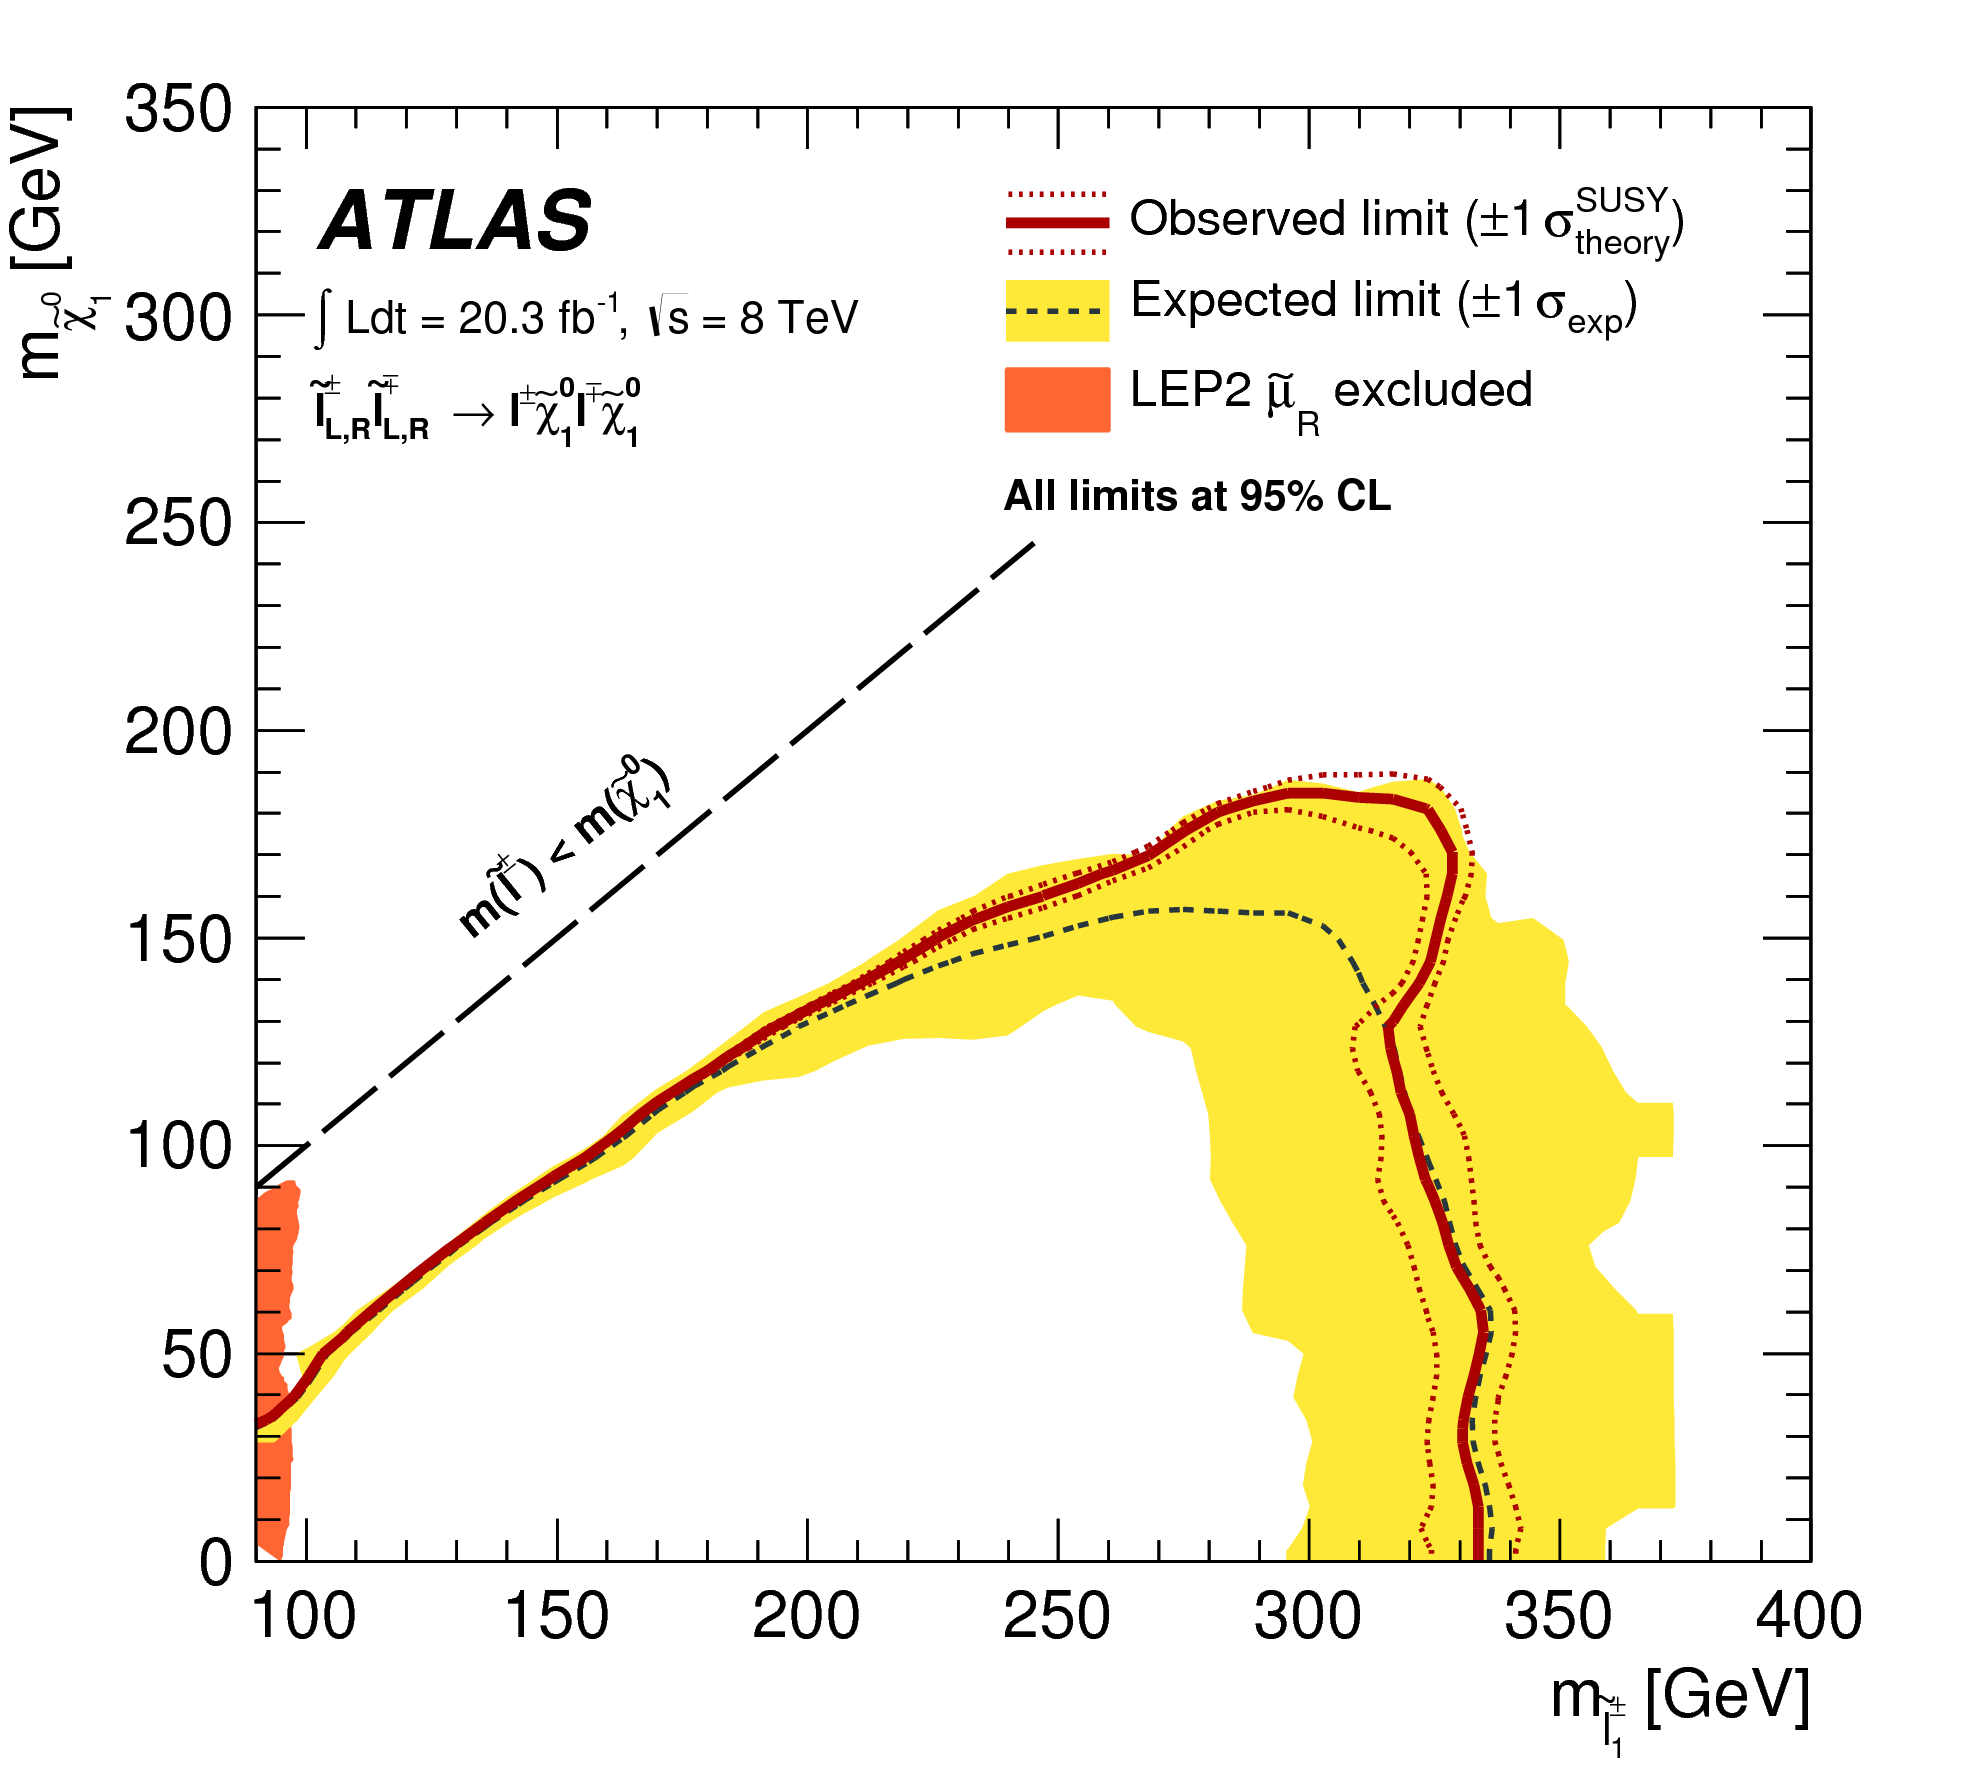
\includegraphics[scale=0.1]{Run1exclusion.png}
\caption{Exclusion limits on mass degenerate left- and right-handed sleptons from ATLAS at 
$8$ TeV \cite{ATLAS:2014}.}
\label{fig:ATLAS 8TeV}
\end{center}
\end{figure}  

Much of the same can also be said about the limits at $13$ TeV, shown in Figure \ref{fig:ATLAS 13TeV}, 
which were presented at the LHCP conference in May 2017. The green area is the previous limit at $8$ 
TeV, while the red on is the new observed limit. For this search a so-called simplified model is used, 
where the only free parameters are $m_{\tilde{\ell}}$ and $m_{\tilde{\chi}_1^0}$. It is noteworthy 
that, although the limits are extended by quite a bit, the limits in the compressed region (i.e.  
small $\Delta m$) aren't improved at all compared to the $8$ TeV search.        

\begin{figure}
\begin{center}
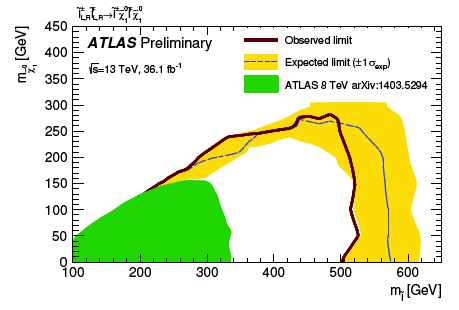
\includegraphics[scale=0.5]{Run2exclusion_new.png}
\caption{Exclusion limits on mass degenerate left- and right-handed sleptons from ATLAS at $13$ TeV 
\cite{ATLAS:2017}.}
\label{fig:ATLAS 13TeV}
\end{center}
\end{figure}

One might wonder why LEP, after all these years, still has better limits than the LHC experiments in the 
compressed region, and there is in fact a very specific reason for this. ATLAS (and CMS) are primarily 
designed 
to search for new (heavy) particles. Such particles should, when decaying, lead to final state particles 
with high transverse momentum ($p_T$). The ATLAS detector is therefore designed to only keep events where 
such particles are present, and the trigger system \cite{ATLAS triggers} in ATLAS is really efficient 
only for leptons with $p_T \gtrsim 20$ GeV. Scenarios with low $\Delta m$ will typically lead to final 
states with so-called \textit{soft} leptons (i.e. low $p_T$), which are hard to study with ATLAS, hence 
sensitivities to such scenarios are low. LEP was on the other hand a precision machine, making it more 
suitable for reaching also the compressed region, but not covering as large parts of the parameter 
space as the LHC. 

However, a study done in ref. \cite{Compressed sleptons} shows that the LHC at $14$ TeV with $100$ 
fb$^{-1}$ of data could be sensitive to $\Delta m$'s as low as $3$ GeV up to 
$m_{\tilde{\ell}_L} \approx 150$ GeV. This study does not make use of the traditional 
technique of studying final states with $\ell^+ \ell^-$ and $\slashed{E}_T$, but uses of events with 
energetic jets from initial state radiation (ISR). The idea is that the produced sleptons will recoil 
against these jets, giving final state leptons with high $p_T$ also in low $\Delta m$ scenarios.        

\section{Summary and conclusions}

We have in this article tried to summarize the current status of slepton searches in particle 
colliders, with focus on selectrons and smuons. We have seen that different experiments have used 
different constrained or simplified models for interpretation of the analysis results, which makes it 
quite hard to directly compare the limits from different experiments.   

We have seen that the ATLAS experiment has excluded a quite large area of the 
$m_{\tilde{\ell}}-m_{\tilde{\chi}_1^0}$ parameter space, while the most general limits with respect 
to the MSSM are actually set by LEP. The lower limit on mass of the right-handed selectron is as 
low as $73$ GeV (i.e. lighter than the $W$-boson), which somewhat answers the question imposed in 
the title of this article. However, stricter limits (or discoveries?) can possibly be made with the
LHC in the future.   

%\newpage

\begin{thebibliography}{9}

% Please take references when possible from SPIRES
% http://inspirehep.net/

\bibitem{Lecture notes} 
  P. Batzing, A. Raklev (2017). \\
  \href{http://www.uio.no/studier/emner/matnat/fys/FYS5190/h17/resurser/notes\_final.pdf}
  {http://www.uio.no/studier/emner/matnat/fys/\\FYS5190/h17/resurser/notes\_final.pdf} 

\bibitem{Constrained models} 
  A. Djouadi et al. (1999). \\
  \href{https://arxiv.org/abs/hep-ph/9901246}{https://arxiv.org/abs/hep-ph/9901246}

\bibitem{Simplified models} 
  J. Alwall et al. (2009), Phys.Rev. D79. \\
  \href{http://inspirehep.net/record/800273}{http://inspirehep.net/record/800273}

\bibitem{PDG}
  C. Patrignani et al. (2017), Chin. Phys. C, 40. \\ 
  \href{http://pdg.lbl.gov/2017/listings/rpp2017-list-supersymmetric-part-searches.pdf}
  {http://pdg.lbl.gov/2017/listings/rpp2017-list-\\supersymmetric-part-searches.pdf}	

\bibitem{ALEPH:2002}
  A. Heister et al. (2002), Phys.Lett. B544, 73-88. 
  \href{https://inspirehep.net/record/591226}{https://inspirehep.net/record/591226}
 
\bibitem{DELPHI:2003} 
  J. Abdallah et al. (2003), Eur.Phys.J.C31, 421-479. 
  \href{http://inspirehep.net/record/632738}{http://inspirehep.net/record/632738}	

\bibitem{ATLAS:2014} 
  G. Aad et al. (2014), JHEP 1405 071. \\
  \href{https://inspirehep.net/record/1286761}{https://inspirehep.net/record/1286761}

\bibitem{ATLAS:2017} 
  ATLAS Collaboration (2017), CONF-SUSY-2017-039. 
  \href{http://cds.cern.ch/record/2267406}{http://cds.cern.ch/record/2267406}      

\bibitem{ATLAS triggers}
  ATLAS Collaboration (2016). \\
  \href{https://arxiv.org/abs/1611.09661}{https://arxiv.org/abs/1611.09661}   

\bibitem{Compressed sleptons}
  A. Barr, J. Scoville (2015). \\ 
  \href{https://arxiv.org/abs/1501.02511}{https://arxiv.org/abs/1501.02511}
 
\end{thebibliography}

\end{document}
